\chapter{Analysis of performed simulations}
The simulations described in this chapter were run in a program prepared for the thesis and the resulting data are available in the project code repository \cite{SimulationsResults}.

\section{Simulation 1}
In this scenario there were only rabbits and plenty of food. The rabbits therefore had ideal conditions to thrive, without the threat of predators and with good availability of food and water.
\subsection{Initial state of the environment}
\begin{description}
    \item[Number of agents]: 4 (2 male rabbits, 2 female rabbits)
    \item[Number of food generators]: 6
\end{description}

\begin{figure}[H]
    \centering
    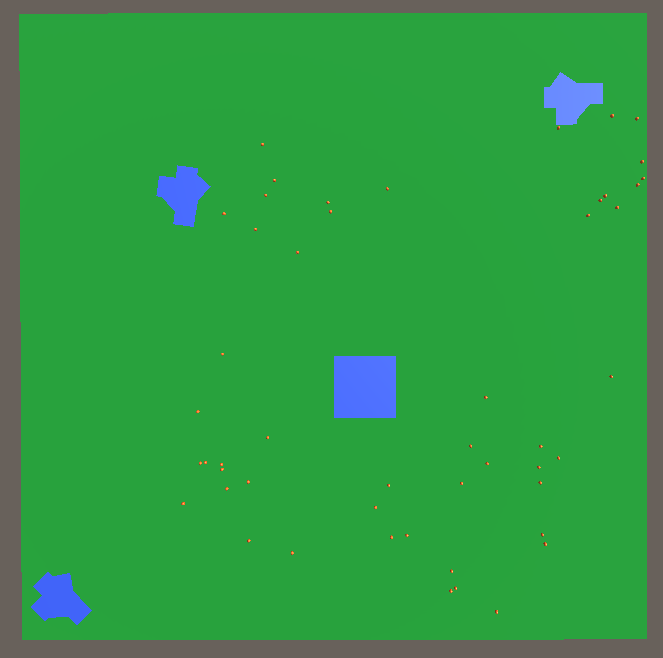
\includegraphics[width=7cm]{Images/Area_Simulation_7_only_rabbits_lot_of_food.png}
    \caption{Distribution of environmental components for Simulation 1.}
    \label{fig:simulation1EnvLayout}
\end{figure}

\subsection{Results}

\begin{figure}[H]
    \centering
    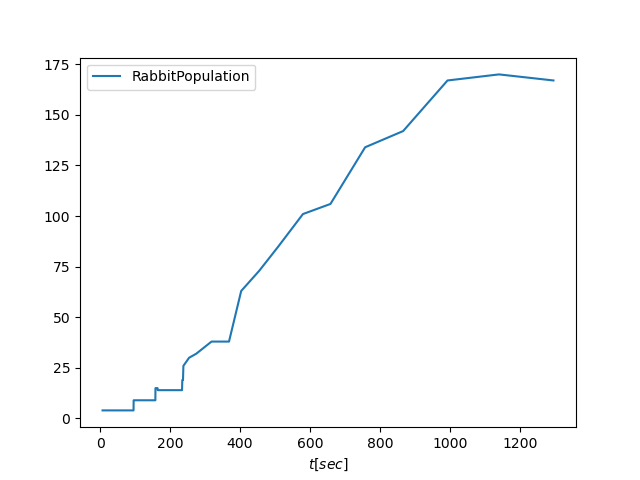
\includegraphics[width=0.9\textwidth]{Images/SimulationResults/Simulation_7_RabbitPopulation.png}
    \caption{Population of rabbits over time.}
    \label{fig:simulation1RabbitPopulation}
\end{figure}

\begin{figure}[H]
    \centering
    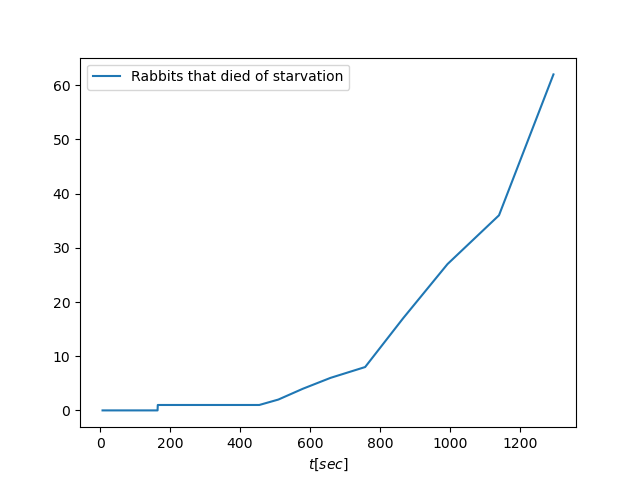
\includegraphics[width=0.9\textwidth]{Images/SimulationResults/Simulation_7_Rabbits that died of starvation.png}
    \caption{Number of rabbits that died of starvation over time.}
    \label{fig:simulation1RabbitsDiedOfHunger}
\end{figure}

\subsection{Analysis}
\subsubsection{Population}
As might be expected, in an environment ideal for rabbits to thrive, their numbers grew rapidly until the number of carrots in the environment was no longer sufficient for the rabbits to survive, then their numbers remained constant. 

\subsubsection{Features}

The graphs of the features over time were not very extensive, their values did not change, so only their final values are worth analysing. The median features of the rabbits at the end of simulation were as follows:
\begin{itemize}
    \item Speed: 74
    \item Sensory range: 85
    \item Fertility: 36
\end{itemize}

As we can see, the value of the fertility feature is not high, from which we can conclude that rapid reproduction was not crucial in this scenario. The speed was quite high, the faster the rabbits could get to the carrots the better chance they had that no other individual would eat it before him. It is interesting to note that the size of the sensor range is really large, despite the fact that in this case the rabbits did not derive any benefit from it because there were no foxes in the environment. The reason could be that there was not much generation of agents in such a one, old rabbits that had an unfavourable trait value in these conditions survived anyway, passing on their genes to their offspring.

\section{Simulation 2}
In this scenario, as in the previous one, there are no predators, but the amount of food is much lower, so that the rabbits will have to compete among themselves for resources in order to survive.
\subsection{Initial state of the environment}
\begin{description}
    \item[Number of agents]: 6 (3 male rabbits, 3 female rabbits)
    \item[Number of food generators]: 1, but with changed parameters:
    \begin{itemize}
        \item spawn interval: 10, instead of 8
        \item spawning radius: 15, instead of 10
        \item plant limit 20: instead of 10
    \end{itemize}
\end{description}

\begin{figure}[H]
    \centering
    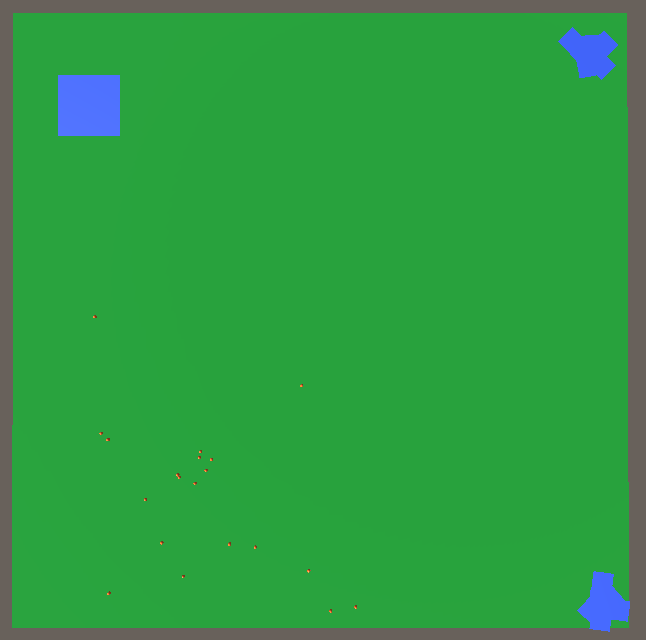
\includegraphics[width=7cm]{Images/Area_Simulation_4_small_amount_of_food.png}
    \caption{Distribution of environmental components for Simulation 2.}
    \label{fig:simulation2EnvLayout}
\end{figure}
    
\subsection{Results}

\begin{figure}[H]
    \centering
    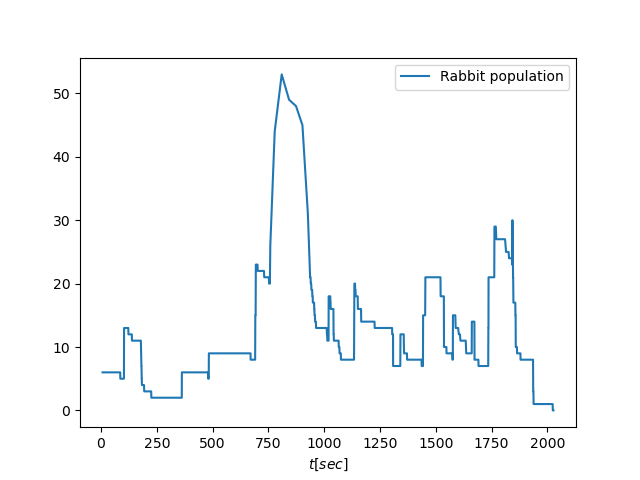
\includegraphics[width=0.9\textwidth]{Images/SimulationResults/Simulation_4_Rabbit population.png}
    \caption{Population of rabbits over time.}
    \label{fig:simulation2RabbitPopulation}
\end{figure}

\begin{figure}[H]
    \centering
    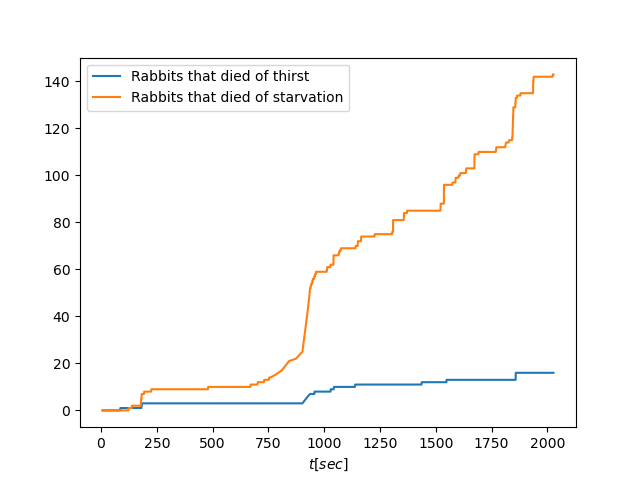
\includegraphics[width=0.9\textwidth]{Images/SimulationResults/Simulation_4_Rabbits that died of thirst_Rabbits that died of starvation.png}
    \caption{Death cause.}
    \label{fig:simulation2RabbitsDiedOfHunger}
\end{figure}

\begin{figure}[H]
    \centering
    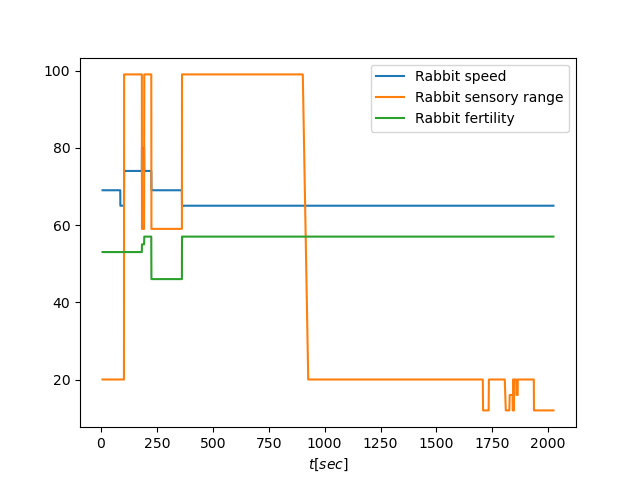
\includegraphics[width=0.9\textwidth]{Images/SimulationResults/Simulation_4_Rabbit speed_Rabbit sensory range_Rabbit fertility.png}
    \caption{Median value of features over time.}
    \label{fig:simulation2FeaturesMedian}
\end{figure}

\subsection{Analysis}
\subsubsection{Population}
In this scenario, initially the rabbits also reproduced rapidly, as can be seen with a maximum at around 800 seconds. At this point, however, the food ran out and the rabbits began to die out just as quickly, as can also be clearly seen in \autoref{fig:simulation2RabbitsDiedOfHunger}. Thereafter, their population fluctuated erratically until there were enough rabbits to eat almost all the food again, leading to the extinction of the entire species.

\subsubsection{Death causes}
As might be expected, most deaths were due to starvation. It is possible to note a sharp rise around the 900th second, corresponding to the extinction of a large proportion of rabbits, after the supply of carrots was no longer sufficient for the growing rabbit population. Thereafter, the function of deceased rabbits over time was linear, corresponding to a period of fluctuation in the rabbit population until the whole species became extinct.

\subsubsection{Features}
Unlike the previous scenario, in this case the rotation of individuals was much higher, allowing for better evolution of traits. Their final values were as follows:
\begin{itemize}
    \item Speed: 65
    \item Sensory range: 12
    \item Fertility: 57
\end{itemize}
The values for speed and fertility seem to be a quite reasonable compromise, reaching values sufficient for survival in the environment, but not too high to justify the high energy consumption that a high value for these traits brings. Whereas the sensory range value, as expected, is low, because in this scenario it does not bring any benefit to the rabbits, but only results in higher energy consumption.

\section{Simulation 3}
In this scenario, the amount of food is at a comfortable level for the rabbits, but there are predators in the environment that prey on them.
\subsection{Initial state of the environment}
\begin{description}
    \item[Number of agents]: 10 (4 male rabbits, 4 female rabbits, 1 male fox, 1 female fox)
    \item[Number of food generators]: 5
\end{description}

\begin{figure}[H]
    \centering
    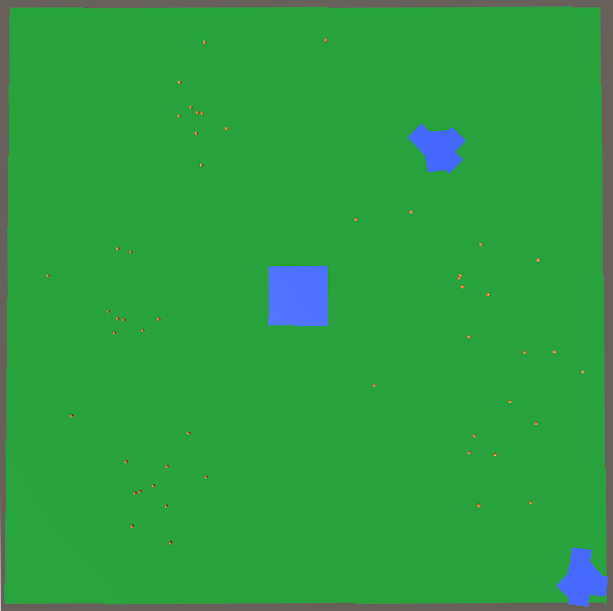
\includegraphics[width=7cm]{Images/Area_Simulation_5_and_6_with_foxes.png}
    \caption{Distribution of environmental components for Simulation 3 and 4.}
    \label{fig:simulation3EnvLayout}
\end{figure}
    
\subsection{Results}

\begin{figure}[H]
    \centering
    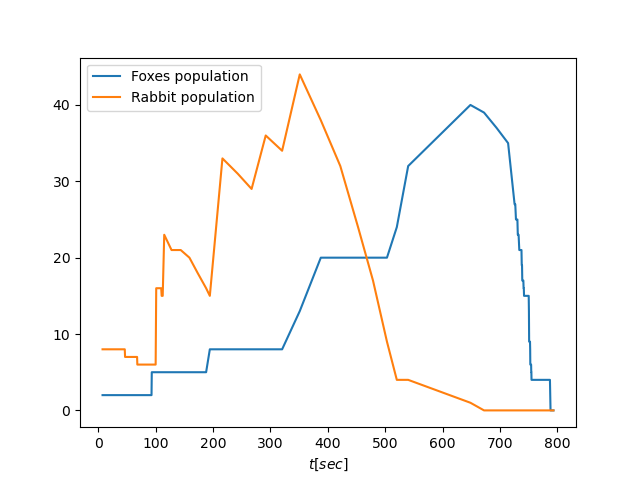
\includegraphics[width=0.9\textwidth]{Images/SimulationResults/Simulation_5_Foxes population_Rabbit population.png}
    \caption{Populations of agents over time.}
    \label{fig:simulation3Pupulations}
\end{figure}

\begin{figure}[H]
    \centering
    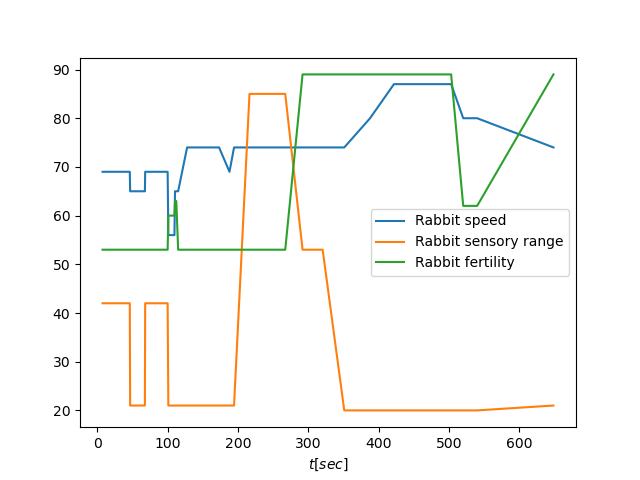
\includegraphics[width=0.9\textwidth]{Images/SimulationResults/Simulation_5_Rabbit speed_Rabbit sensory range_Rabbit fertility.png}
    \caption{Median value of rabbit features over time.}
    \label{fig:simulation3RabbitFeaturesMedian}
\end{figure}

\begin{figure}[H]
    \centering
    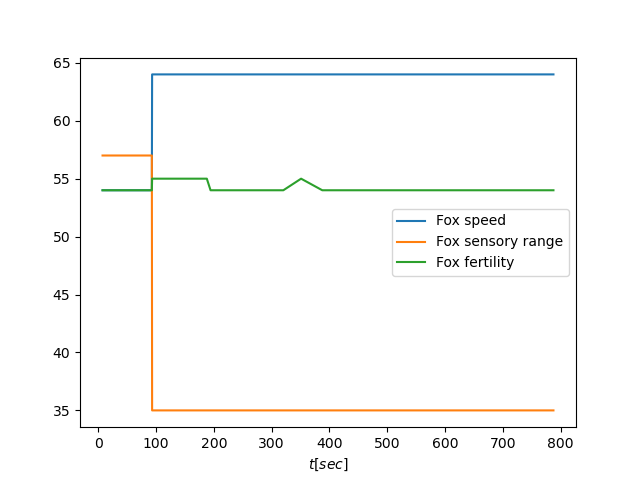
\includegraphics[width=0.9\textwidth]{Images/SimulationResults/Simulation_5_Fox speed_Fox sensory range_Fox fertility.png}
    \caption{Median value of fox features over time.}
    \label{fig:simulation3FoxFeaturesMedian}
\end{figure}

\begin{figure}[H]
    \centering
    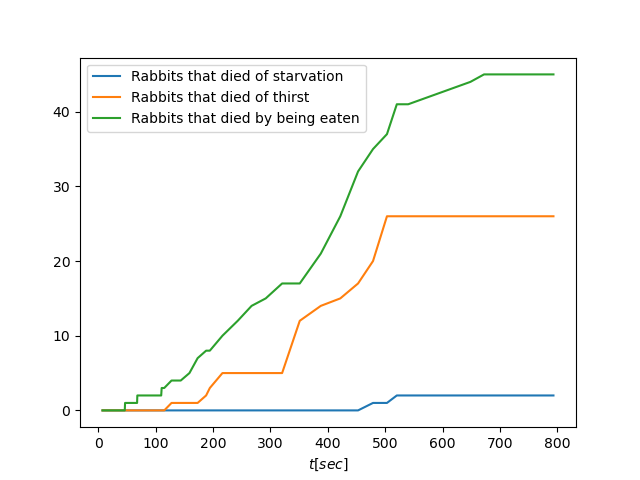
\includegraphics[width=0.9\textwidth]{Images/SimulationResults/Simulation_5_Rabbits that died of starvation_Rabbits that died of thirst_Rabbits that died by being eaten.png}
    \caption{Rabbits death cause.}
    \label{fig:simulation3RabbitDeathCause}
\end{figure}

\begin{figure}[H]
    \centering
    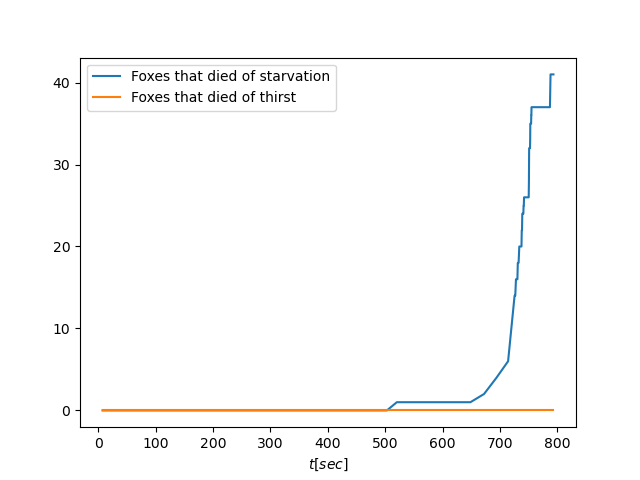
\includegraphics[width=0.9\textwidth]{Images/SimulationResults/Simulation_5_Foxes that died of starvation_Foxes that died of thirst.png}
    \caption{Foxes death cause.}
    \label{fig:simulation3FoxDeathCause}
\end{figure}

\subsection{Analysis}
\subsubsection{Population}
As in previous scenarios, the rabbit population initially shot up. But then, due to the fact that it was an ideal opportunity for the foxes to thrive as they had food and drink in abundance, the situation reversed. At around second 350, the fox population started to rise strongly, while the rabbit population fell very sharply. However, with this rapid growth, the foxes sealed their own fate, because it led to the extinction of the entire rabbit population. For a while, foxes with their needs satisfied multiplied even more, until they ran out of food and they, too, began to die out rapidly. So a strong correlation can be seen between the two species and how prosperity can easily turn into inhospitable conditions.

\subsubsection{Death causes}
Most rabbits were obviously eaten by foxes, but quite a few deaths were also caused by thirst. On the other hand, no fox died of thirst. This was most probably due to the fact that the foxes, by staying at the watering holes, scared away the rabbits, which were afraid to approach the predators. Therefore, the foxes not only actively contributed to the extinction of the rabbits by eating them, but also passively cut off their access to water.

\subsubsection{Features}
In the case of rabbits, we see dynamically changing feature values, actively striving towards the most favourable values for rabbits in this environment. The features that were more valuable to the rabbits were fertility, and speed, as can be seen when the values of these features reached very high scores in the later stages of the simulation. Interestingly, sensory range apparently did not give the rabbits enough of an advantage to make it profitable to bear its genetic cost. 

In contrast, for foxes, the values remained virtually the same throughout most of the simulations. This may be due to the fact that individuals of this species only started dying out towards the end, so the same genes were in the gene pool all the time. For the less adapted individuals, the environment was favourable enough for them to survive anyway, giving them the opportunity to pass on their weak genes to their offspring.

\newpage
\section{Simulation 4}
\label{Simulation4}
This scenario is no different from the previous one, but the simulation went differently.
\subsection{Initial state of the environment}
The environment is exactly the same as the previous one.

\subsection{Results}

\begin{figure}[H]
    \centering
    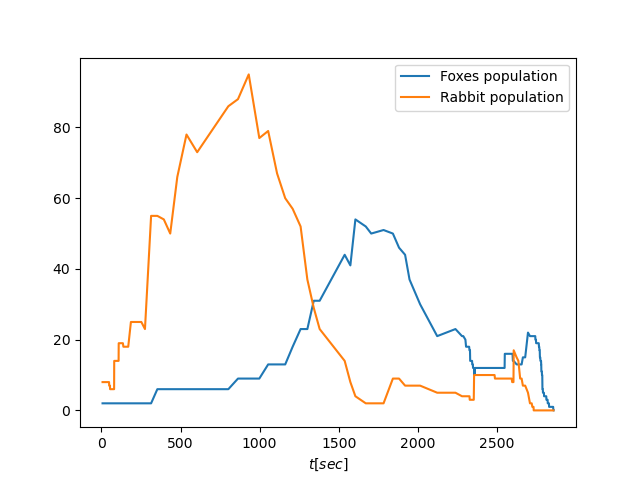
\includegraphics[width=0.9\textwidth]{Images/SimulationResults/Simulation_6_Foxes population_Rabbit population.png}
    \caption{Populations of agents over time.}
    \label{fig:simulation4Pupulations}
\end{figure}

\begin{figure}[H]
    \centering
    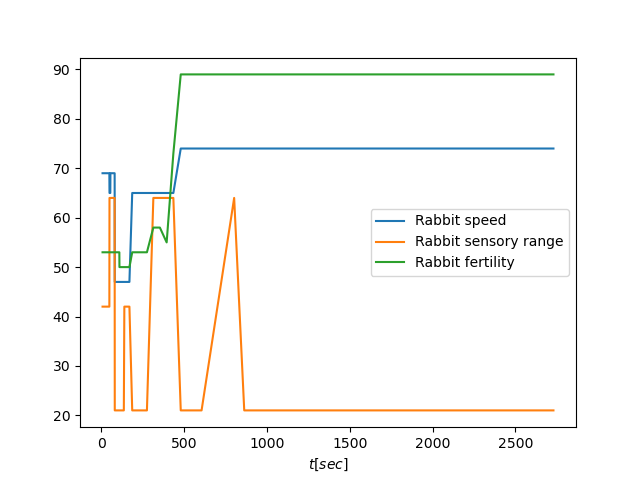
\includegraphics[width=0.9\textwidth]{Images/SimulationResults/Simulation_6_Rabbit speed_Rabbit sensory range_Rabbit fertility.png}
    \caption{Median value of rabbit features over time.}
    \label{fig:simulation4RabbitFeaturesMedian}
\end{figure}

\begin{figure}[H]
    \centering
    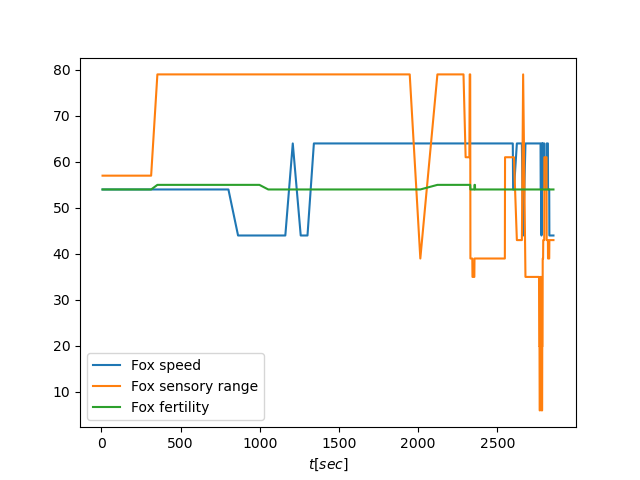
\includegraphics[width=0.9\textwidth]{Images/SimulationResults/Simulation_6_Fox speed_Fox sensory range_Fox fertility.png}
    \caption{Median value of fox features over time.}
    \label{fig:simulation4FoxFeaturesMedian}
\end{figure}

\begin{figure}[H]
    \centering
    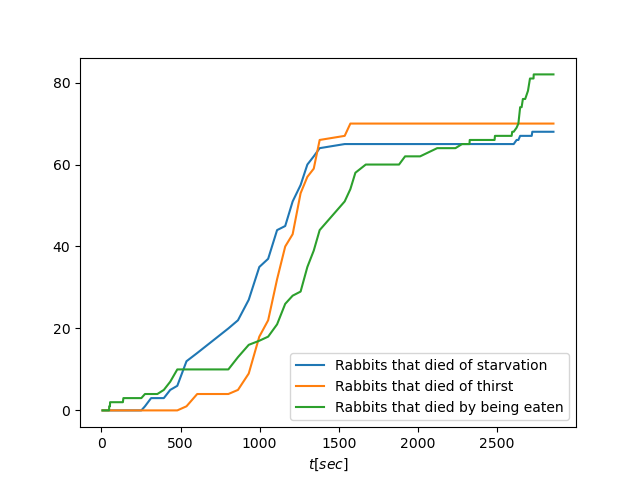
\includegraphics[width=0.9\textwidth]{Images/SimulationResults/Simulation_6_Rabbits that died of starvation_Rabbits that died of thirst_Rabbits that died by being eaten.png}
    \caption{Rabbits death cause.}
    \label{fig:simulation4RabbitDeathCause}
\end{figure}

\begin{figure}[H]
    \centering
    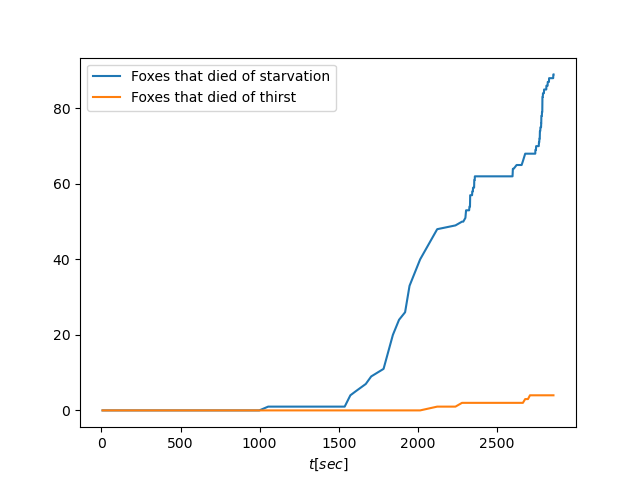
\includegraphics[width=0.9\textwidth]{Images/SimulationResults/Simulation_6_Foxes that died of starvation_Foxes that died of thirst.png}
    \caption{Foxes death cause.}
    \label{fig:simulation4FoxDeathCause}
\end{figure}

\subsection{Analysis}
\subsubsection{Population}
In this scenario, as in the previous one, once the foxes had eaten a large proportion of the rabbits, they themselves began to starve to death. However, this time a few rabbits managed to survive and multiply again, but the foxes quickly dealt with them, this time finally. However, a certain cyclicality can be observed, if the rabbits had started to breed later, more foxes would have died out and they could have rebuilt their population more by reaching the same environmental state as originally (however with different, more adapted trait values nonetheless).

\subsubsection{Death causes}
Because the leaves started reproducing later than in the previous simulation, this led to more deaths from starvation, which were previously much lower. This time it had values similar to death from thirst and being eaten by a predator. In this simulation the availability of carrots started to play a role again, there were not enough carrots in the environment to satisfy such a growing population of rabbits.

\subsubsection{Features}
The dominant feature values for rabbits were established at the very beginning, where the weakest individuals were immediately eaten by the foxes. This led to a state where rabbits had a genetic advantage over foxes for most of the simulations, which was most likely the reason that foxes reproduced more slowly than in the previous simulation. 

The features of foxes began to develop rapidly towards the end of the simulation, when foxes began to die out and only strong individuals could survive in this difficult environment. The final values of the features are as follows: 
\begin{itemize}
    \item Speed: 44
    \item Sensory range: 43
    \item Fertility: 54
\end{itemize}
Thus, it can be seen that for foxes each of the traits was important, but they could not afford their high values. 